\section{Analysis (Example usage)}
\label{sec:analysis}

In this section, we'll showcase the ability of our dataset and our analysis tools to study questions we think may be of interest to privacy policy regulators. Our tool does not identify causal relationships, but it can be used to flag particular relationships for deeper investigation.

\subsection{Self-regulation bodies}
Many companies exist to offer ``privacy seals,'' or certifications of compliance with privacy standards. These companies arguably serve a self-regulatory purpose--many industries regulate themselves through central, industry-run bodies\rnote{Cite? Confirm?}.

We've searched our data for several privacy seal companies, listed in table \ref{tbl:sealcomps}. We measured how frequently each company name appears by searching the entities extracted by SpaCy. For each company, we've also listed the interval with the highest number of occurrences, and how many occurrences there were in that interval.
\rnote{TODO get interval}

\begin{table}
\begin{tabular}{c|c|c} 
    Company & Maximum Occurrence & Interval\\
    \hline
    BBBOnLine & 10 & ~\\
    CNIL & 76 & ~\\
    ePrivacy & 20 & ~\\
    EuroPriSe & 0 & ~\\
    TrustArc & 1838 & ~\\
    VeraSafe & 49 & ~\\
    WebTrust & 2 & ~\\
\end{tabular}\label{tbl:sealcomps} 
\caption{A table of privacy seal companies and the maximum number of websites containing the name of the company over all intervals. In 2017, TRUSTe changed their name to TrustArc\cite{trustetrustarc}. To account for the name change, we changed all references of ``TRUSTe'' to ``TrustArc.''}
\end{table}

Of these companies, only TrustArc was flagged by our analysis methods, so we will focus deeper on TrustArc. We can track the usage of the term ``TrustArc'' in our entity set, as we show in figure \ref{fig:trustarc}.  The results suggest that TrustArc has declined in popularity, and the lack of a replacement indicates that no non-governmental authority currently exists to self-regulate industry privacy policies. Even at its height, TrustArc was only present on slightly over 3\% of websites, suggesting self-regulation authorities have minimal impact on the privacy policy landscape.

\rnote{Combine these figures}
\begin{figure}
    \centering
    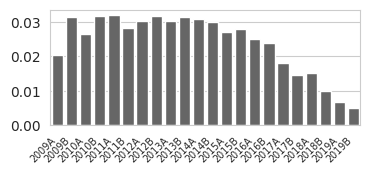
\includegraphics[width=0.45\textwidth]{figures/trustarc-total}
    \caption{The adoption of the ``TrustArc'' or ``TRUSTe'', counted by websites, normalized per interval. Notice the usage is relatively stable, and begins to drop in 2015. Today, usage has dropped significantly.} %https://privacypolicies.cs.princeton.edu/policies/metrics/LOCAL_2_POS_GROWTH/e-grams_top_LOCAL_2_POS_GROWTH_unique_NP_NR_MS_CL.html
    \label{fig:trustarc}
\end{figure}

\begin{figure}
    \centering
    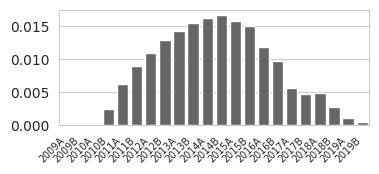
\includegraphics[width=0.45\textwidth]{figures/privacyseal}
    \caption{The adoption of the term ``Privacy Seal'', counted by unique policies, normalized per interval. Notice the bell-shaped curve with a peak in the latter half of 2014B.} %https://privacypolicies.cs.princeton.edu/policies/metrics/LOCAL_2_POS_GROWTH/e-grams_top_LOCAL_2_POS_GROWTH_unique_NP_NR_MS_CL.html
    \label{fig:privacyseal}
\end{figure}

One of TrustArc's major products was the TRUSTe Privacy Seal. We can track the term ``Privacy Seal'' as a named entity through time, as seen in figure \ref{fig:privacyseal}. This may capture other privacy seals, if present. Regardless, we can see that ``Privacy Seal'' occurs with diminishing frequency, almost vanishing in the latter half of 2019. This is not surprising, given our previous discussion about the decline in TrustArc and the lack of other privacy seal companies. 

\subsection{Discussion of tracking technologies}
Tracking of users on the internet has become a hot topic in recent years. One theory of regulation suggests that regulators should bar specific technologies. Another theory suggests that proper disclosure to consumers is adequate. While our methods cannot directly test disclosure, we can measure how tracking terminology usage has changed overtime.\rnote{Someone really needs to heavily edit this paragraph}

We'll explore selected terms highlighted by our methods to better understand whether companies reliably disclose their practices. We've broken the terms we've found into four categories: tracking terminology, figure \rnote{fig?}; tracking phrases, figure \rnote{fig?}; tracking organizations, figure \rnote{fig?}; and tracking technologies, figure \rnote{fig?}.

As we can see.... \rnote{todo}

\rnote{Tracking terminology}

advertising

marketing

data

\rnote{Tracking phrases}

information we collect from you
we do not sell trade
usage data
aggregated data

\rnote{Trackers}

instagram
shopify
amazon web services
facebook
DART
mailchimp

\rnote{Tracking technology}

web beacon
cookie
flash
cross-device
fingerprinting

\rnote{Start writing analysis now -- use placeholder graphs and variables for e.g. policy count}

Start from a research question, then try to extract answers from \\
Drop topic models\\

Privacy seal question is a great question to look into\\
Talk to Mihir \& Jonathan about phrases\\

Does disclosure work?\cite{marotta2019does} \\

Present some things we found

Show that we can extract key events

Subject ``best metric''\\
Subjective ``worst metric''\\
What will be useful for consumers/users?\\

Think about how to present this
